\chapter{位置推定}
\thispagestyle{empty}
\label{chap4}
\minitoc

\newpage
%%%%%%%%%%%%%%%%%%%%%%%%%%%%%%%%%%%%%%%%%%%%%%%%%%%%%%%%%%%%%%%%%%%%%%%%%%%%%%%
%==============================================================================
% 4.1
%==============================================================================
\section{はじめに}

本章では,位置$\bm{P}$を推定する手法について述べる.

4.2節にて,手法の概要について述べる.

4.3節にて,特徴量の計算について述べる.

4.4節にて,$xy$座標の推定方法について述べる.

4.5節にて,$z$座標の推定方法について述べる.


\clearpage
%==============================================================================
% 4.2
%==============================================================================
\section{位置推定の概要}

位置推定では,各エッジ点とそれに対応する単位球面勾配ベクトル,姿勢$\bm{O}$,ラインマップからカメラの位置$\bm{P}$を推定する.
図\ref{fig:derotation}に示すように,ワールド座標系から姿勢$\bm{O}$の分ずれているカメラ座標系$x_{\rm{sph}}y_{\rm{sph}}z_{\rm{sph}}$を$\bm{O}^{-1}$回転させることでワールド座標系と向きが一致した状態に変換して位置を推定する.変換後のカメラ座標系を$x'_{\rm{sph}}y'_{\rm{sph}}z'_{\rm{sph}}$とする.
\\

\begin{figure}[b]
 \begin{center}
 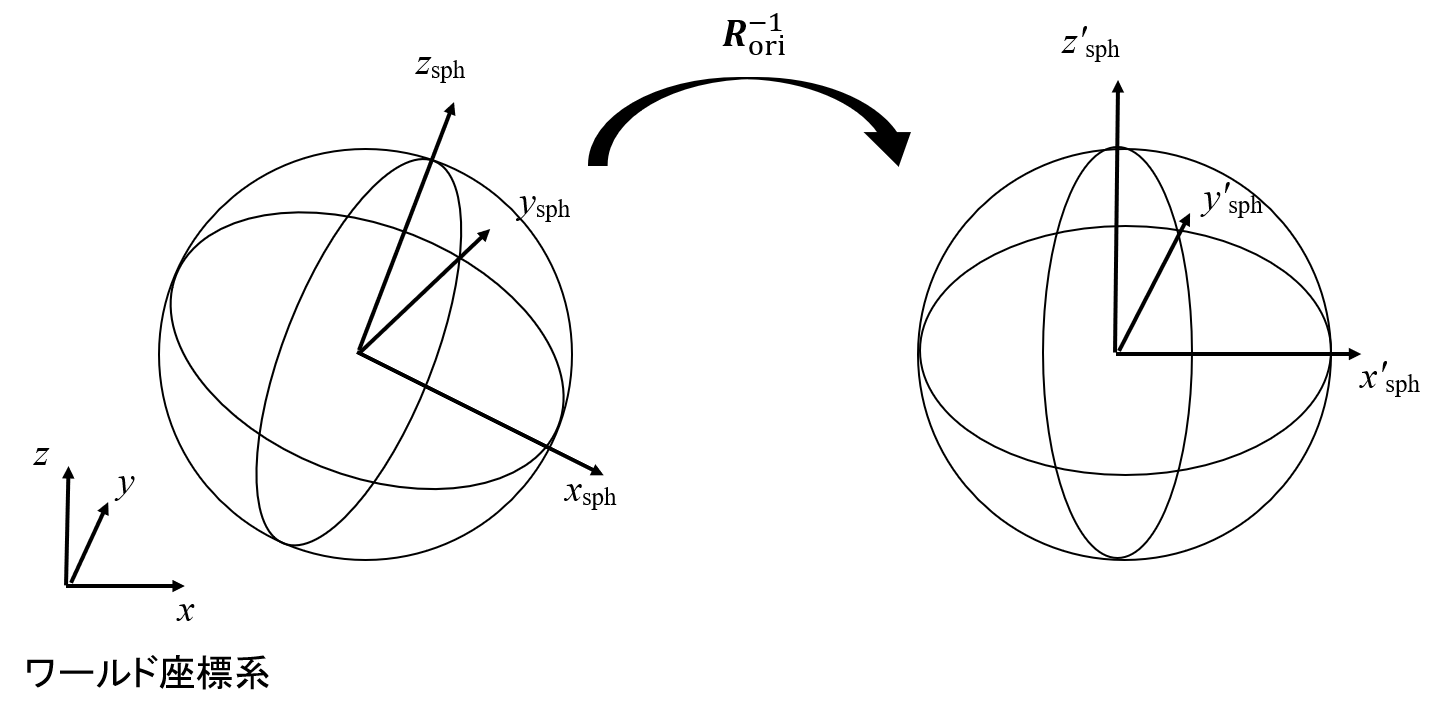
\includegraphics[width=0.85\columnwidth]{./chap4/fig/derotation.png}
 \caption{ワールド座標系の向きと一致させるようなカメラ座標系の回転}
 \label{fig:derotation}
 \end{center}
\end{figure}

位置推定では,ワールド座標系における各軸方向の直線が球面に投影されたとき,それぞれの軸方向を法線ベクトルとする大円と交わる点の分布を特徴量とする.
この特徴量は,$y'_{\rm{sph}}z'_{\rm{sph}}$平面,$x'_{\rm{sph}}z'_{\rm{sph}}$平面,$x'_{\rm{sph}}y'_{\rm{sph}}$平面のそれぞれにおける単位円上の点の集合で表される.
例えば,図\ref{fig:feature_x}に示すように,青い実線で示す$x$軸方向に伸びる直線は青い破線で示す線のように球面に投影され,この破線と$x'_{\rm{sph}}$方向を法線ベクトルとする大円の交点は$y'_{\rm{sph}}z'_{\rm{sph}}$平面における単位円上に存在する.
すべての$x$軸方向の直線について同様に交点を計算すると,$y'_{\rm{sph}}z'_{\rm{sph}}$平面における単位円上の点の集合が得られる.
これと同様に,$y$軸方向に伸びる直線から$x'_{\rm{sph}}z'_{\rm{sph}}$平面における単位円上の点の集合が得られ(図\ref{fig:feature_y}),$z$軸方向に伸びる直線から$x'_{\rm{sph}}y'_{\rm{sph}}$平面における単位円上の点の集合が得られる(図\ref{fig:feature_z}).
これらをそれぞれ,$yz$特徴量,$xz$特徴量,$xy$特徴量と呼ぶ.
これらの特徴量は各カメラ位置において一意に定まるため,推定する画像の特徴量とラインマップから計算する各位置における特徴量を比較し,最も類似度の高い位置を探索することによりカメラの位置を推定することができる.
\\

\begin{figure}[tb]
 \begin{center}
 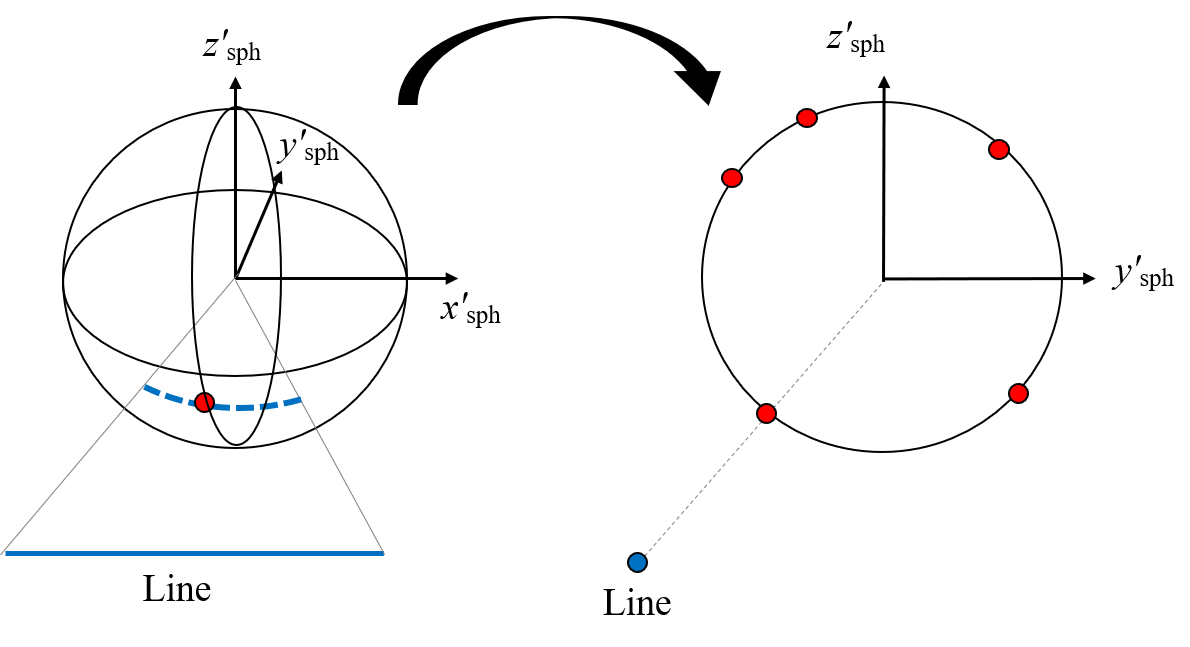
\includegraphics[width=0.85\columnwidth]{./chap4/fig/feature_x.png}
 \caption{$x$軸方向の直線から得られる$y'_{\rm{sph}}z'_{\rm{sph}}$平面における単位円上の点の集合}
 \label{fig:feature_x}
 \end{center}
\end{figure}

\begin{figure}[tb]
 \begin{center}
 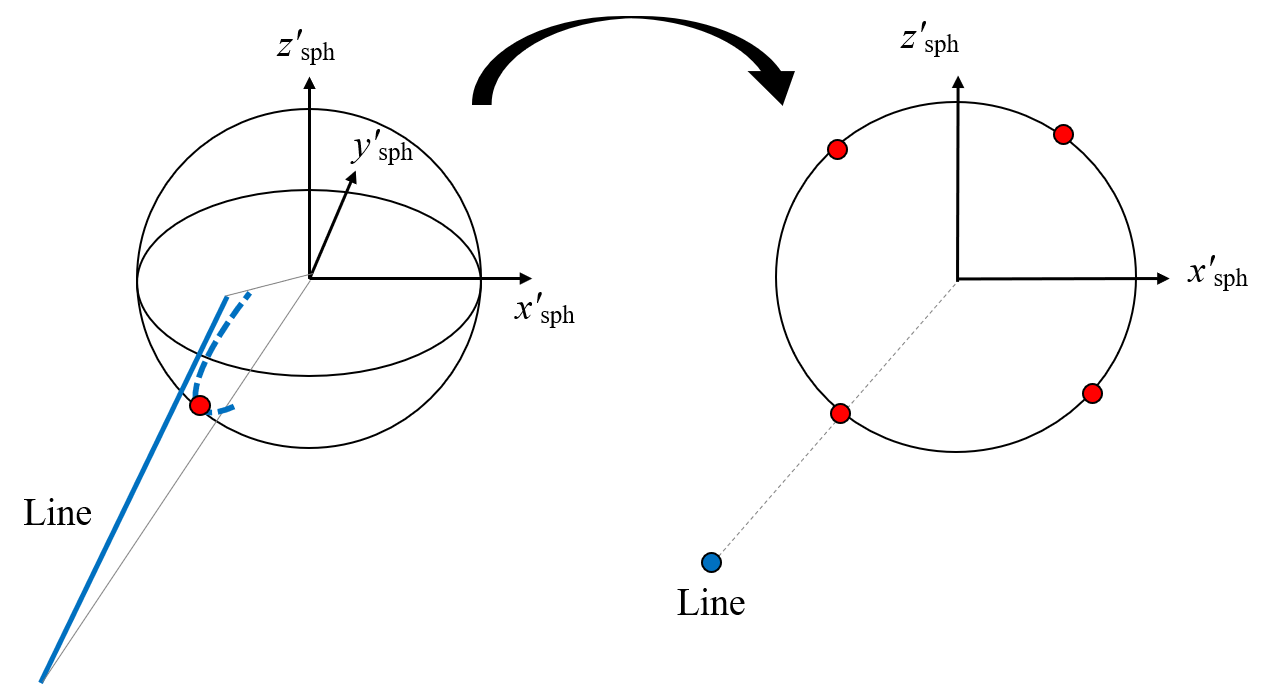
\includegraphics[width=0.85\columnwidth]{./chap4/fig/feature_y.png}
 \caption{$y$軸方向の直線から得られる$x'_{\rm{sph}}z'_{\rm{sph}}$平面における単位円上の点の集合}
 \label{fig:feature_y}
 \end{center}
\end{figure}

\clearpage

\begin{figure}[tb]
 \begin{center}
 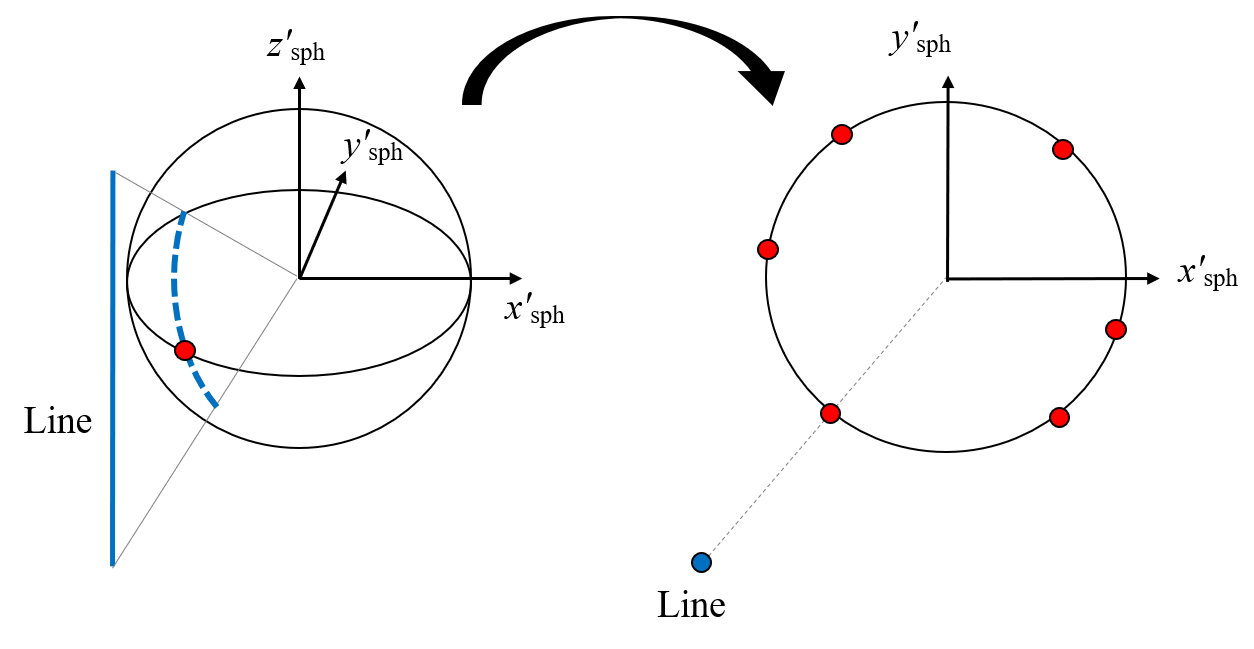
\includegraphics[width=0.85\columnwidth]{./chap4/fig/feature_z.png}
 \caption{$z$軸方向の直線から得られる$x'_{\rm{sph}}y'_{\rm{sph}}$平面における単位円上の点の集合}
 \label{fig:feature_z}
 \end{center}
\end{figure}


ここで,各軸方向の直線から得られる特徴量は,その軸方向のカメラ移動に依存せずに定まる.
つまり,$x$軸方向の直線から得られる$yz$特徴量はカメラの$yz$座標にのみにより定まり,$y$軸方向の直線から得られる$xz$特徴量はカメラの$xz$座標にのみにより定まり,$z$軸方向の直線から得られる$xy$特徴量はカメラの$xy$座標にのみにより定まる.
これを利用して,はじめに1つの特徴量を用いて2自由度の推定を行い,次に残りの特徴量から1つを選んで残りの1自由度の推定を行うことで,2自由度の推定と1自由度の推定に分離して行う.
本研究では,はじめに$xy$特徴量を用いた2次元の探索により$xy$座標を推定し,その後$xz$特徴量と推定された$x$座標を用いた1次元の探索により$z$座標を推定した.
\\

位置推定の流れを図\ref{fig:flow4}に示す.
まず,各エッジ点とそれに対応する単位球面勾配ベクトル,姿勢$\bm{O}$から推定する画像の特徴量を計算し,$xy$特徴量と$xz$特徴量を得る.
次に,得られた$xy$特徴量とラインマップから$xy$座標の推定を行い,推定値$x^*,\ y^*$を求める.
最後に,$xz$特徴量,推定値$x^*$,ラインマップから$z$座標の推定を行い,推定値$z^*$を求める.
以上の流れで,カメラの位置$\bm{P}$の推定値$\bm{P}^*=[x^*,\ y^*,\ z^*]^{\mathrm{T}}$を得る.


\begin{figure}[tb]
 \begin{center}
 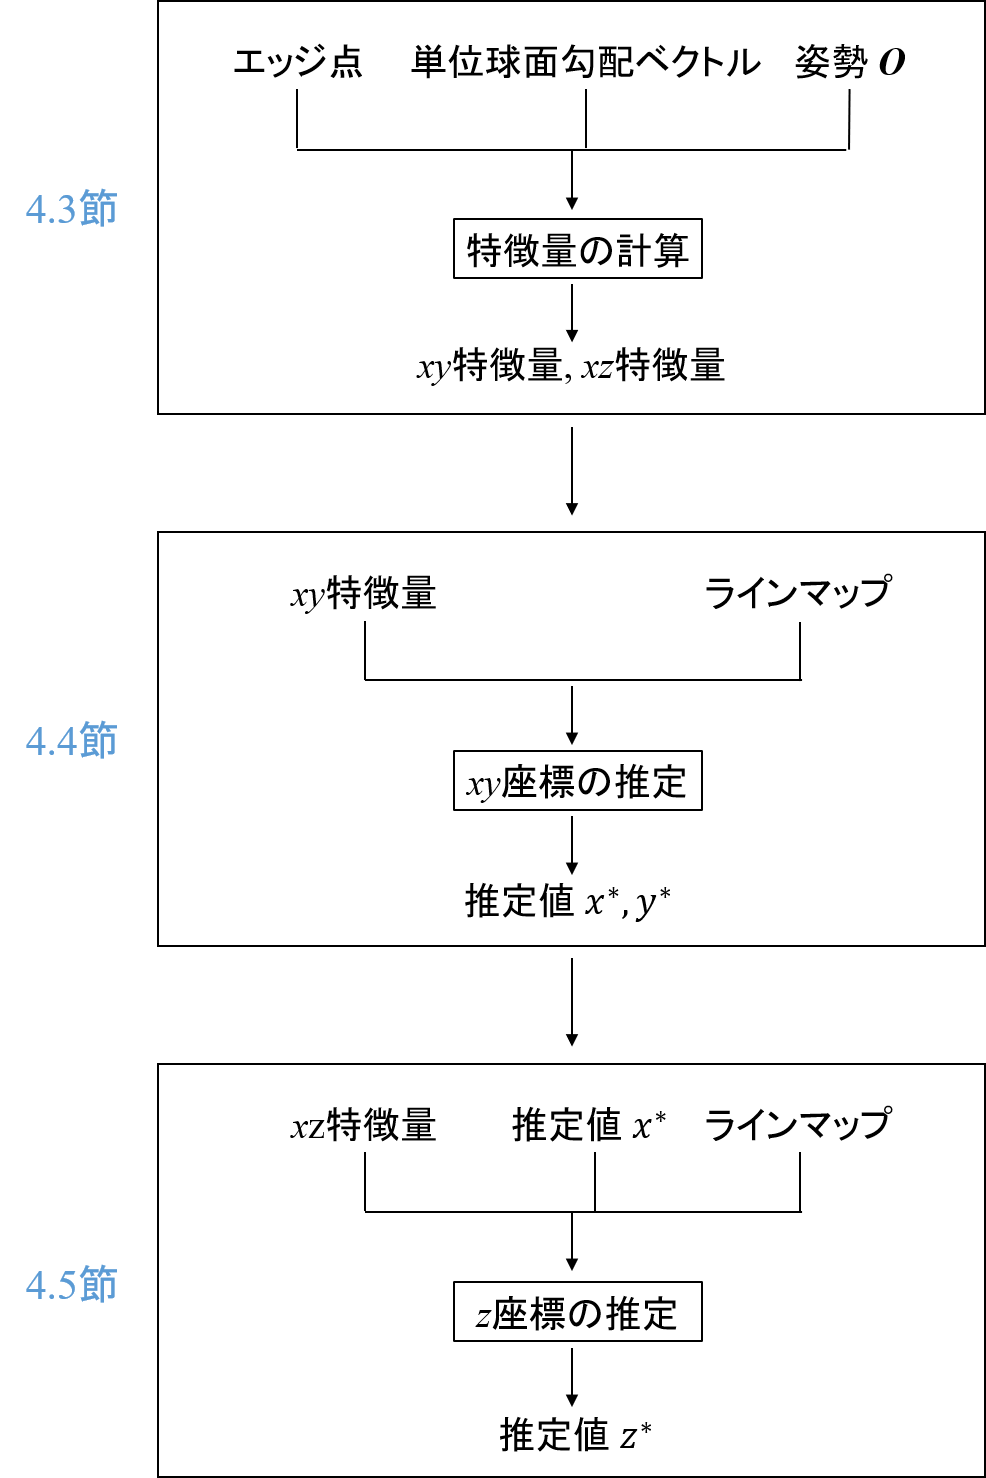
\includegraphics[width=0.7\columnwidth]{./chap4/fig/flow4.png}
 \vspace{5mm}
 \caption{位置推定の流れ}
 \label{fig:flow4}
 \end{center}
\end{figure}

\clearpage
%==============================================================================
% 4.3
%==============================================================================
\section{特徴量の計算}

\subsection{エッジ点の分類}

エッジ点とそれに対応する単位球面勾配ベクトルの組から$xy$特徴及び$xz$特徴量を得るためには,それぞれの勾配ベクトルがどの軸方向の直線によるエッジ点から得られたものかによって分類する必要がある.
姿勢を推定したあと,3平面のうち最も近い平面からの距離が閾値以上の単位勾配ベクトルをoutlierとして除去する.
残った単位球面勾配ベクトルをそれぞれ最も近い平面ごとに分類することで,元の入力画像におけるエッジ点を,どの方向の直線に属するものかで3つのグループに分類する.
分類されたエッジ点の例を図\ref{fig:classified}に示す.
赤色のエッジ点が$x$軸方向の直線によるエッジ点,緑色のエッジ点が$y$軸方向の直線によるエッジ点,青色のエッジ点が$z$軸方向の直線によるエッジ点をそれぞれ表している.
\\

\begin{figure}[b]
 \begin{center}
 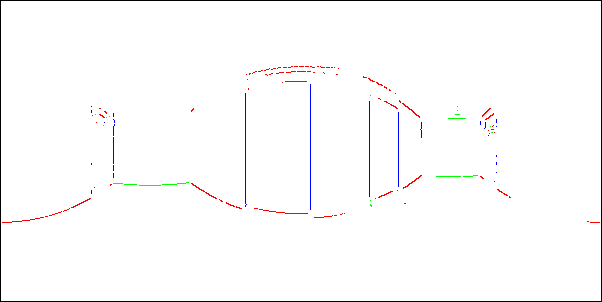
\includegraphics[width=0.7\columnwidth]{./chap4/fig/edge_inlier.png}
 \caption{分類されたエッジ点}
 \label{fig:classified}
 \end{center}
\end{figure}

\clearpage

\subsection{$xy$特徴量}

$xy$座標の推定に用いる$xy$特徴量には,$z$軸方向の直線が球上に投影される直線と全天球カメラの$x_{sph}y_{sph}$平面の交点の分布$(x_k,y_k)\ (k=1, 2,..., n)$を用いる.
特徴量の計算では,4.3.1項で分類したエッジ点のうち,$z$軸方向の直線に属するものを抽出して行う.
図\ref{fig:classified}に青色で示されたエッジ点がこれに該当する.
図\ref{fig:feature_xy}に示すように,抽出されたエッジ点座標を$(u_k, v_k)\ (k=1, 2,..., n)$,画像の幅を$w$とすると,交点$(x_k,y_k)$は以下の式によって求められる.

\begin{equation}
   \left(x_k,\ y_k\right) = \left(-\sin\frac{2\pi u_k}{w},\ -\cos\frac{2\pi u_k}{w}\right).
\end{equation}

\begin{figure}[b]
 \begin{center}
 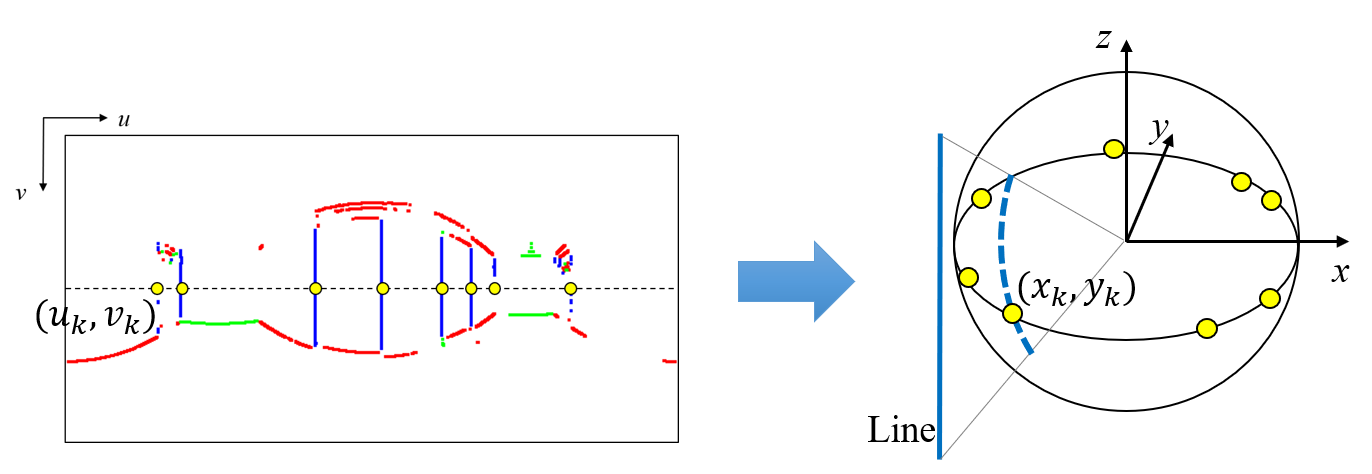
\includegraphics[width=1.0\columnwidth]{./chap4/fig/feature_xy.png}
 \vspace{5mm}
 \caption{$xy$特徴量($x_{sph}y_{sph}$平面)の計算}
 \label{fig:feature_xy}
 \end{center}
\end{figure}

\clearpage
\subsection{$xz$特徴量}
$z$座標の推定に用いる$xz$特徴量には,$y$軸方向の直線が球上に投影される直線と全天球カメラの$x_{sph}z_{sph}$平面の交点の分布$(x_k,z_k)\ (k=1, 2,..., n)$を用いる.
まず,図\ref{fig:classified}に示すエッジ画像を$x$軸回りに-90 deg回転させることで,図\ref{fig:rotated_edge}のようなエッジ画像に変換する.
特徴量の計算では,このエッジ画像内のエッジ点のうち,$y$軸方向の直線に属するものを抽出して行う.
図\ref{fig:rotated_edge}に緑色で示されたエッジ点がこれに該当する.
図\ref{fig:feature_xz}に示すように,抽出されたエッジ点座標を$(u_k, v_k)\ (k=1, 2,..., n)$,画像の幅を$w$ pixelとすると,交点$(x_k,z_k)$は以下の式によって求められる.

\begin{equation}
   \left(x_k,\ z_k\right) = \left(-\sin\frac{2\pi u_k}{w},\ -\cos\frac{2\pi u_k}{w}\right).
\end{equation}

\begin{figure}[b]
 \begin{center}
 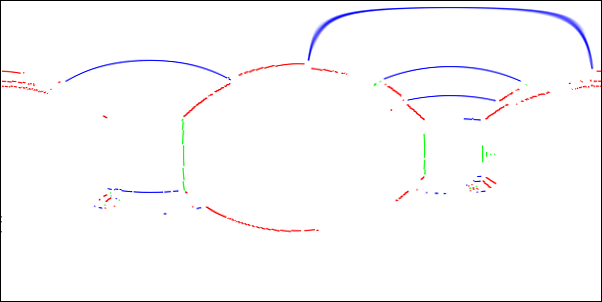
\includegraphics[width=0.7\columnwidth]{./chap4/fig/rotated_edge.png}
 \vspace{5mm}
 \caption{$x$軸回りに-90 deg回転させたエッジ画像}
 \label{fig:rotated_edge}
 \end{center}
\end{figure}


\begin{figure}[b]
 \begin{center}
 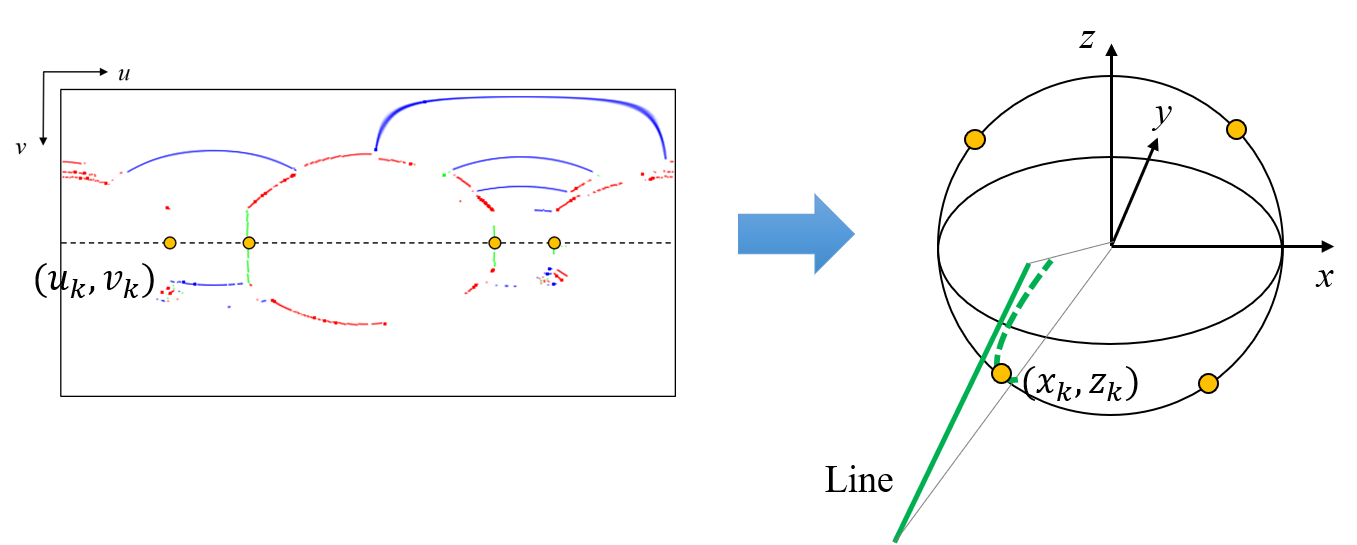
\includegraphics[width=1.0\columnwidth]{./chap4/fig/feature_xz.png}
 \vspace{5mm}
 \caption{$xz$特徴量($x_{sph}z_{sph}$平面)の計算}
 \label{fig:feature_xz}
 \end{center}
\end{figure}


\clearpage
%==============================================================================
% 4.4
%==============================================================================
\section{$xy$座標の推定}

$xy$座標の推定では,$z$座標を固定し,2次元の最適化によって推定する.
図\ref{fig:search_xy}に座標$(x,y)$における全天球カメラを上から見た図を示す.
緑色の点が上記の方法で求めた交点,赤色の点がラインマップから求めた,座標$(x,y)$から遮蔽されることなく見えるz軸方向の直線をそれぞれ表している.
画像から全ての直線を検出できるとは限らないため交点と直線の数は必ずしも一致せず,交点の数を$n$,直線の数を$m$とする.
各交点と直線の距離を,全天球カメラ座標系においてそれぞれが成す角によって定義し,すべての交点に対する最も近い直線までの距離の二乗和が最小となるような座標$(x,y)$を推定値とする.
交点の座標を$(x_k,y_k)\ (k=1, 2,..., n)$,ラインマップにおける$z$軸方向の直線の$xy$座標を$(x_l, y_l)\ (l=1, 2,...,m)$とすると,これらの距離$d_{k,l}$は,以下の式で得られる.
\begin{equation}
   d_{k,l} = \cos^{-1}\left(\frac{x_k(x_l-x)+y_k(y_l-y)}{\sqrt{(x_l-x)^2+(y_l-y)^2}}\right).
\end{equation}

$d_{k,l}\ (l=1,2,...,m)$のうち,最も小さいものを$d_k$とする.

\begin{equation}
   d_k = \min\left(d_{k,1},\ d_{k,2},\cdots,\ d_{k,m}\right).
\end{equation}

全ての交点における$d_k$の二乗和を最小とするようなパラメータ$(x^*,y^*)$が,$xy$座標の推定値である.
この非線形最適化を,Levenberg-Marquardt法を用いて解く.

\begin{equation}
(x^*,y^*)=\argmin_{x,y} \sum_{k=1}^nd_k^2.
\label{eq:optim2}
\end{equation}

\begin{figure}[b]
 \begin{center}
 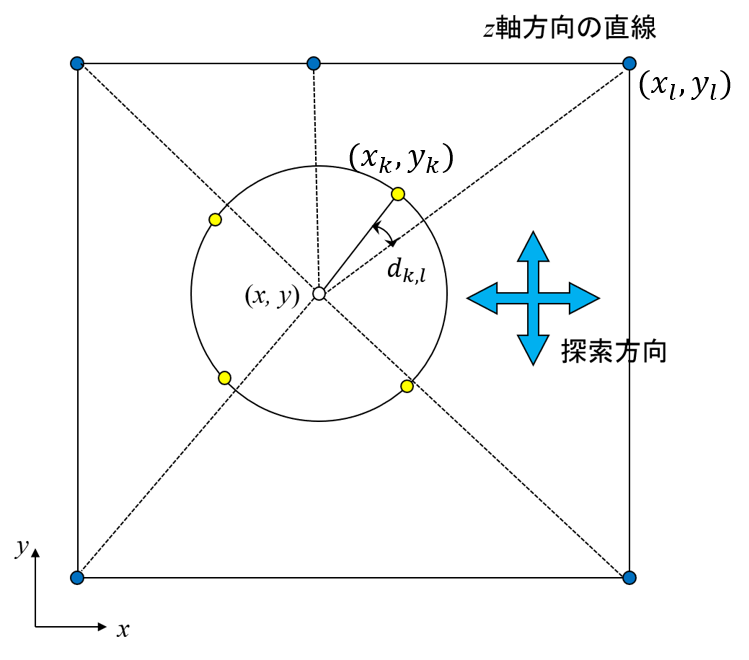
\includegraphics[width=0.6\columnwidth]{./chap4/fig/search_xy.png}
 \caption{座標$(x,y)$における全天球カメラを$z$軸方向から見た図}
 \label{fig:search_xy}
 \end{center}
\end{figure}


\clearpage
%==============================================================================
% 4.4
%==============================================================================
\section{$z$座標の推定}

$z$座標の推定では,$y$座標と前節で推定した$x$座標を固定し,1次元の最適化によって推定する.
まず,$xy$座標の推定と同様に,各交点$(x_k,z_k)$と$y$軸方向の直線の$xz$座標$(x_l,z_l)\ (l=1,2,...,m)$に対して以下の式で距離を計算する.

\begin{equation}
   d_{k,l} = \cos^{-1}\left(\frac{x_k(x_l-x^*)+z_k(z_l-z)}{\sqrt{(x_z-x^*)^2+(z_l-z)^2}}\right).
\end{equation}

$d_{k,l}\ (l=1,2,...,m)$のうち,最も小さいものを$d_k$とする.

\begin{equation}
   d_k = \min\left(d_{k,1},\ d_{k,2},\cdots,\ d_{k,m}\right).
\end{equation}

全ての交点における$d_k$の二乗和を最小とするようなパラメータ$(z^*)$が,$z$座標の推定値である.
この非線形最適化を,Levenberg-Marquardt法を用いて解く.

\begin{equation}
(z^*)=\argmin_{z} \sum_{k=1}^nd_k^2.
\label{eq:optim2}
\end{equation}


\begin{figure}[b]
 \begin{center}
 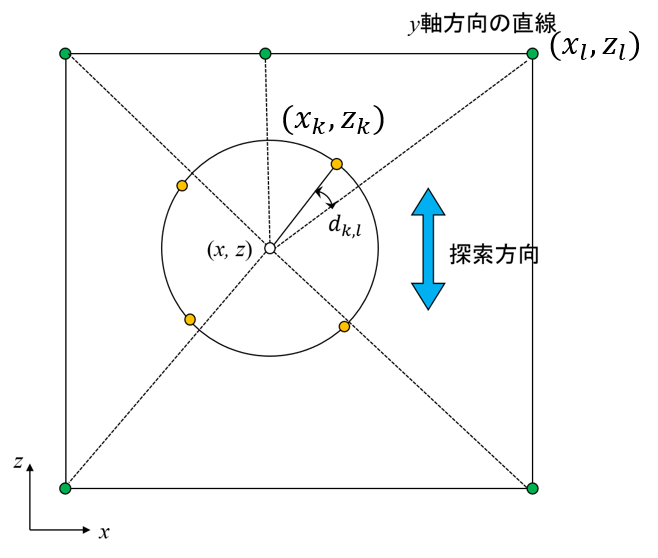
\includegraphics[width=0.6\columnwidth]{./chap4/fig/search_xz.png}
 \caption{座標$(x,z)$における全天球カメラを$y$軸方向から見た図}
 \label{fig:search_xz}
 \end{center}
\end{figure}


\clearpage
%==============================================================================
% 4.5
%==============================================================================
\section{おわりに}

本章では,位置推定手法について説明した.

4.2節にて,位置推定の概要を述べた.

4.3節にて,特徴量の計算について述べた.

4.4節にて,$xy$座標の推定方法について述べた.

4.5節にて,$z$座標の推定方法について述べる.


次章では,提案手法の有効性を検証するために行った実験について述べる.

\clearpage
%%%%%%%%%%%%%%%%%%%%%%%%%%%%%%%%%%%%%%%%%%%%%%%%%%%%%%%%%%%%%%%%%%%%%%%%%%%%%%%%%
%%%%% Local Variables:
%%%%% mode: katex
%%%%% TeX-master: "../thesis"
%%%%% End:
